\section{Methods}

\subsection{Banner similarities}
When connecting a device to the internet, it needs to be configured. The installer needs competence to do this properly, and to spend time to perform the installation. To make such devices more accessible and efficient, finished solutions are most often used. Due to this, the same devices mostly have the same default configuration, and therefore the same banners. This can be used to identify devices within the chosen constraints by using the following method.
\begin{enumerate}
    \item Identify a device fulfil the constraints and is connected to the internet.
    \item Find the IP address of said device, and find its Shodan entry.
    \item Get its banner.
    \item Use unique information from the banner to find all devices with similar banners.
\end{enumerate}
The most difficult of these steps is to find the IP address. The easiest way to do this is to own a device and find its IP address. Unfortunately, this project does not have access to any devices that fit the constraints set.
If this is not an option, the device would be found by guessing what information could be found in its banner, for example the device name or ports it has open.


\subsection{Internet Service Provider and IP ranges} \label{sec:isp_method}
Internet Service Providers(ISP) are the organisations that connect people and companies to the internet. ISP charges money to deliver internet connection, and most people have a subscription. While a lot of ISPs are generalized, and deliver the internet to both private and organizational customers, others are more specialized. 
IPv4 addresses are 32 bit, meaning they can range from 0.0.0.0 to 255.255.255.255. The IPv4 addresses are sold to organizations, for them to distribute further. For example, an Internet Service Provider(ISP) will give IPv4 addresses to the customers while they use their subscribed internet connections. This distribution of IPv4 addresses to organizations is illustrated in \cref{fig:ipv4_map}.

\begin{figure} [H]
    \centering
    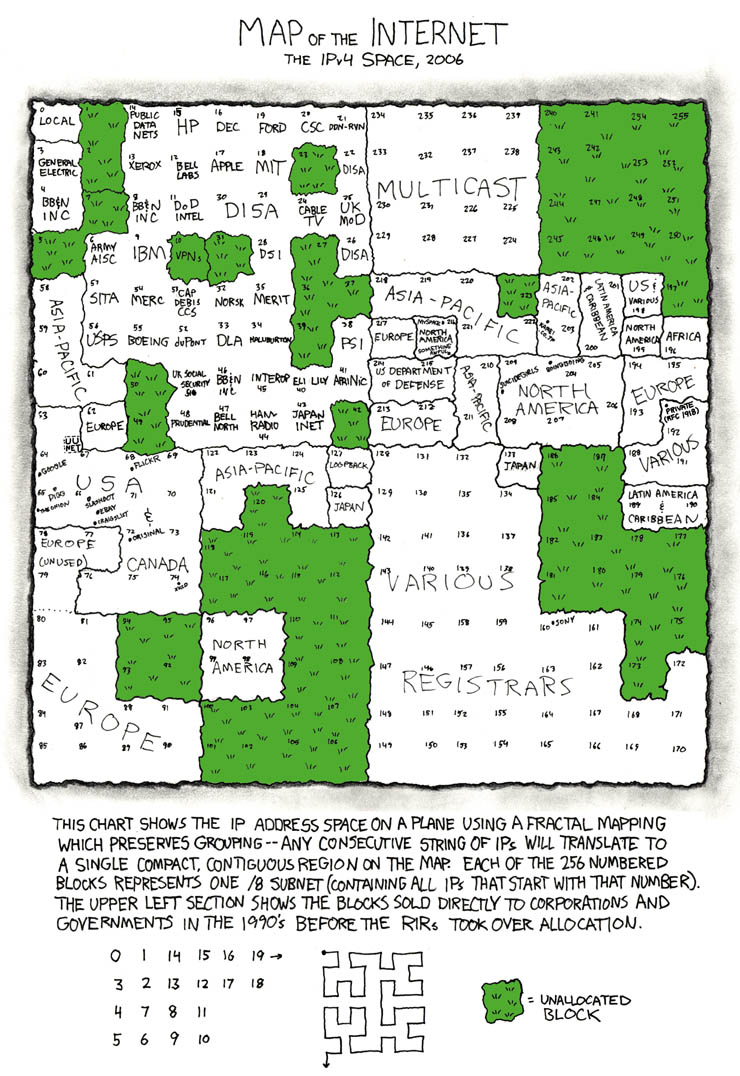
\includegraphics[scale=4]{Figurer/map_of_the_internet.jpg}
    \caption{A map of the IPv4 space, from the XKCD web comic. \cite{xkcd} }
    \label{fig:ipv4_map}
\end{figure}

\subsubsection{Autonomous System}
One or more CIDR blocks that is owned by an organisation and has a single defined routing policy is called an Autonomous System(AS). A typical example of an organisastion that owns an AS, is an Internet Service Provider(ISP). TODO: reference https://tools.ietf.org/html/rfc1930
The AS are registered with unique identification numbers. Online tools, like \href{https://hackertarget.com/as-ip-lookup/}{\textbf{Hackertarget AS-IP lookup}} \cite{asip_lookup}, makes it possible to find the parent AS of an IP address. Then the rest of the IP addresses belonging to the same AS can be found. This is done by using the Shodan "net" filter, which will filter CIDR blocks. The same way as in \cref{sec:isp_method}, for this method to work, the AS must be for a purpose within the project constraints.


\subsection{Reverse IP geolocation}
When Regional Internet Registries (RIR) give IP addresses to organizations, they also register contact information on the IP addresses. A part of this information is a location, specifying a country and city. Some data providers claim that the country accuracy is between 95\% and 99\%, while the city accuracy is between 50\% and 75\%.\cite{geolocation_acc}With accuracy poor, it is not possible to decide if an IP address is within the constraints by using its IP geolocation. The information returned by the one of the RIRs can be seen in \cref{fig:RIPE_NCC}.
Shodan have a filter for the location. This filter can also filter by latitude and longitude. However, I have not been able to find any information on how Shodan gather this information. \todo{Er det innafor å seie "I have" her?} 
Because of these uncertainties, IP geolocation can not be conclusive for finding devices within the constraints. However, by reversing the technique, it would be possible to narrow down the selection of IP addresses by first defining an area. Shodan can use the filter "geo:latitude,longitude,radius" to filter on addresses based on location.  

\begin{figure} [H]
    \centering
    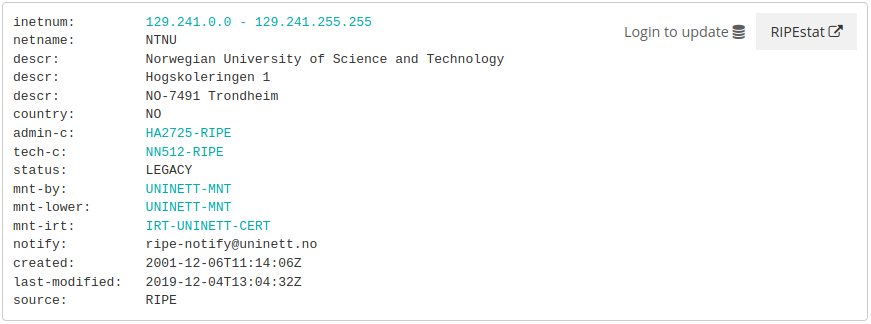
\includegraphics[scale=0.5]{Figurer/ripe.png}
    \caption{The IP address lookup of RIPE NCC \cite{ripe_whois}}
    \label{fig:RIPE_NCC}
\end{figure}

With many major seaports, like Rotterdam, Antwerp and Hamburg, the North Sea has a lot of marine traffic. The sea also has a lot of offshore oil and gas fields; Ekofisk, Sleipner, Forties and Valhall, to mention a few.\cite{oil_field_lists} With this much activity within both constraints, the marine and offshore industries, a lot of things in the area have to be connected to the internet. To test if the IP geolocation services of Shodan could detect devices connected to the internet, a large area of the North sea was chosen: a circle with 270 km around 56\degree24\textquotesingle00.0N 3\degree00\textquotesingle36.0E, as seen in \cref{fig:geolocation}. To use Shodan to find devices within this area, the command \cref{lst:geolocation_sea} was used. As seen in the output from the command, no devices was found within the area.

\begin{figure} [H]
    \centering
    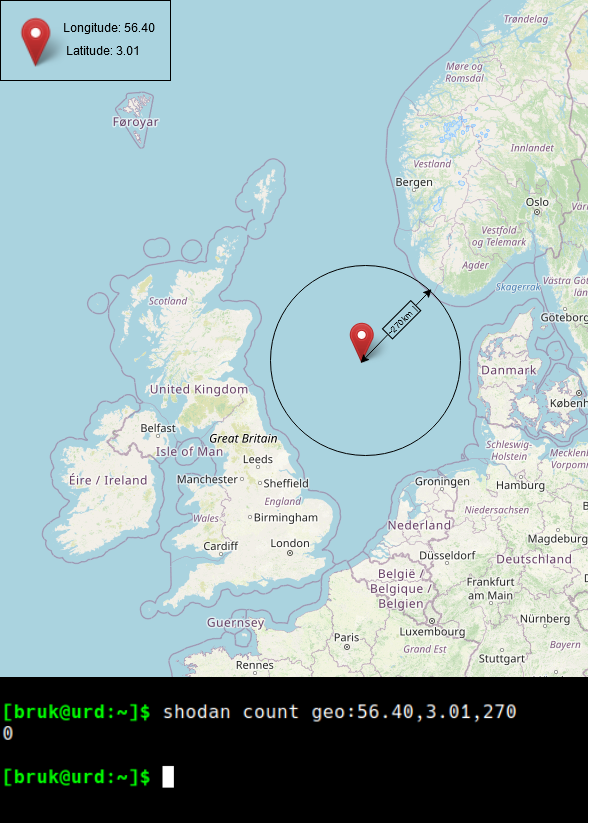
\includegraphics[scale=0.7]{Figurer/geolocation.png}
    \caption{Shodan "geo" filter visualized. Map copyright: https://www.openstreetmap.org/copyright}
    \label{fig:geolocation}
\end{figure}

\subsection{Latency and traceroute}
The simplest form of reaching another device on the internet is called a "ping". This sends a echo request to an IP address, to make it send a response back. It is mostly used to check if a device is reachable. To prevent a bug where packets travel in an infinite loop instead of reaching the recipient, packets have a Time To Live (TTL) counter. This counter increments every time a packet travels trough a switch or router. When this counter is reached, the packet is stopped, and a message is returned to the sender, informing it of the loss.
The "traceroute" command takes advantage of the fact that the Time To Live counter can be set by the sender. It will start the TTL counter at 1 and sending a message towards a predefined target IP address. This message will then travel 1 step towards its target before it is returned. Then it increments this counter and repeats the send. In addition, traceroute will time how long the packet uses before it is returned, called "Round Trip Time"(RTT).
The Round Trip Time can give an idea of how the signal travels. Faster RTT can be because of shorter distance or better infrastructure. On the other hand, slow RTT can indicate farther distance or worse infrastructure.

\section{Problems}
\subsection{NAT}
Due to NAT connecting devices to the internet trough a single router, Shodan will only scan the outer NAT routing device, and not the devices behind the NAT. NAT is not always used for getting more IPv4 addresses. Sometimes it is used purposely to hide IPv4 addresses from the public internet.

\subsection{Obfuscation}


\subsection{Geolocation}
